%
\documentclass{sig-alternate-br}

\usepackage{graphicx}
\usepackage{subfigure,dblfloatfix} %to fix the problem of [h!] [t!] [!b]
\usepackage{caption}

\usepackage[table]{xcolor} 

\usepackage[breaklinks]{hyperref}
\hypersetup{colorlinks, citecolor=blue, filecolor=black, linkcolor=blue, urlcolor=blue}

\usepackage{libs/gantt} %for the planning table
\newcommand\comment[1]{{\sffamily\textbf{[COMMENT: #1]}}}

\begin{document}
%
% --- Author Metadata here --- DO NOT REMOVE OR CHANGE 
\conferenceinfo{13$^{th}$ Twente Student Conference on IT}{June 21$^{st}$, 2010, Enschede, The Netherlands.}
\CopyrightYear{2010} % Allows default copyright year (200X) to be over-ridden - IF NEED BE.
%\crdata{0-12345-67-8/90/01}  % Allows default copyright data (0-89791-88-6/97/05) to be over-ridden - IF NEED BE.
% --- End of Author Metadata ---

\title{Bachelor's Student Conference Proceedings Paper in LaTeX Template}
% In Bachelor Referaat at University of Twente the use of a subtitle is discouraged.
% \subtitle{[Instructions]}

%
% You need the command \numberofauthors to handle the 'placement
% and alignment' of the authors beneath the title.
%
% For aesthetic reasons, we recommend 'three authors at a time'
% i.e. three 'name/affiliation blocks' be placed beneath the title.
%
% NOTE: You are NOT restricted in how many 'rows' of
% "name/affiliations" may appear. We just ask that you restrict
% the number of 'columns' to three.
%
% Because of the available 'opening page real-estate'
% we ask you to refrain from putting more than six authors
% (two rows with three columns) beneath the article title.
% More than six makes the first-page appear very cluttered indeed.
%
% Use the \alignauthor commands to handle the names
% and affiliations for an 'aesthetic maximum' of six authors.
% Add names, affiliations, addresses for
% the seventh etc. author(s) as the argument for the
% \additionalauthors command.
% These 'additional authors' will be output/set for you
% without further effort on your part as the last section in
% the body of your article BEFORE References or any Appendices.

\numberofauthors{3} %  in this sample file, there are a *total*
% of EIGHT authors. SIX appear on the 'first-page' (for formatting
% reasons) and the remaining two appear in the \additionalauthors section.
%
\author{
% You can go ahead and credit any number of authors here,
% e.g. one 'row of three' or two rows (consisting of one row of three
% and a second row of one, two or three).
%
% The command \alignauthor (no curly braces needed) should
% precede each author name, affiliation/snail-mail address and
% e-mail address. Additionally, tag each line of
% affiliation/address with \affaddr, and tag the
% e-mail address with \email.
%
% 1st. author
\alignauthor
1st Author\\
       \affaddr{University of Twente}\\
       \affaddr{P.O. Box 217, 7500AE Enschede}\\
       \affaddr{The Netherlands}\\
       \email{1st author's email address}
% 2nd. author
\alignauthor 2nd Author\\
       \affaddr{2nd author's affiliation}\\
       \affaddr{1st line of address}\\
       \affaddr{2nd line of address}\\
       \email{2nd author's email address}
% 3rd. author
\alignauthor 3rd Author\\
       \affaddr{3rd author's affiliation}\\
       \affaddr{1st line of address}\\
       \affaddr{2nd line of address}\\
       \email{3rd author's email address}
}
% There's nothing stopping you putting the seventh, eighth, etc.
% author on the opening page (as the 'third row') but we ask,
% for aesthetic reasons that you place these 'additional authors'
% in the \additional authors block, viz.
\additionalauthors{Additional authors: John Smith (The
Th{\o}rv{\"a}ld Group, email: {\texttt{jsmith@affiliation.org}})
and Julius P.~Kumquat (The Kumquat Consortium, email:
{\texttt{jpkumquat@consortium.net}}).}
\date{30 July 1999}
% Just remember to make sure that the TOTAL number of authors
% is the number that will appear on the first page PLUS the
% number that will appear in the \additionalauthors section.

\maketitle
\begin{abstract}
In this paper, we describe the formatting guidelines for ACM SIG Proceedings.  
\end{abstract}

% A category with the (minimum) three required fields (NOT USED in Bachelor Referaat)
% \category{H.4}{Information Systems Applications}{Miscellaneous}
%A category including the fourth, optional field follows...
% \category{D.2.8}{Software Engineering}{Metrics}[complexity
% measures, performance measures]

\keywords{Keywords are your own designated keywords.}

\begin{abstract}

\comment{The structure of an average abstract should have the (i) context, (ii) problem, (iii) proposal, and your most astonishing (iv) finding. Your goal is to meet $\pm$100 words. The ``context'' part describes what your reader should know to understand your research. The ``problem'' part describes why your research need to be don; why it is interesting; and why someone needs to spend time reading your work. The ``proposal'' part describes what your approach has different from others. Finally, your ``finding'' part surprises your reader, make him VERY interested to read your paper. In a proposal you ``findings'' part describes what do you expect to be the most astonishing achievement of your research.}

\end{abstract}
\section{Introduction} 
\label{sec:introduction}

\comment{The Introduction section has more or less the same structure as your abstract. The difference is that in the abstract each part is one statement/phrase, while in the introduction each part is a paragraph. So, (i) context, (ii) problem, (iii) proposal, and your most astonishing (iv) finding. Of course in the Introduction section you can give far more details than in the abstract. Avoid to copy and paste statements, re-write with different words.}

\comment{In addition to the structure that you already know you should include your \textit{research questions} between the ``proposal'' paragraph and the ``findings''. The statement that precede the RQ is something like the following: }

``To pursue our goal, we have defined the following research questions (RQ) as the basis of our research: 
\begin{itemize}	
	\item \textbf{RQ1:} What are ..?
	\item \textbf{RQ2:} How to ... ?
	 \item \textbf{RQ3:} How to ...?
\end{itemize}
''

\comment{Please, avoid "yes or no" questions. Make questions that your reader are not able to answer immediately. Usually the questions depend on each other, it means that to answer one question you must answer the one before.}

\comment{Before a little bit of your most astonishing findings you must to introduce the structure of your paper/proposal. Usually the text looks like the following.}
 
``The remainder of this paper/proposal is organized as follows. Section 2 will discuss the approaches expected for answering each research question. After that, we present a preliminary planning for the research questions in Section 3. Finally, we conclude with a proposal and planning for the thesis structure in Section 4.'' 



\section{Related Work}

Go to Google scholar and search using keywords related to your research. Then,
download some paper that the title immediately show similarities with your
research. You must be able to judge the strong and weak-points of each paper.
Also, you can extend your literature study by looking the related work section
of each downloaded paper. In addition to that, you can look who cited the papers
that you decided to include (till this moment) on your research (google scholar
shows this information for you). This step is important because the papers that
cited the paper that you decide to include on your research are potential papers
to include on your section. Note that the final goal of this section is a table
that summarizes the characteristics of each paper and your critical analysis to
highlight the existing gaps of research.

\section{Proposal}

In this part I would like you to add a conceptual figure with your idea (if possible). On this, I must say that Figures MUST be in pdf format (I like to use Inkscape to create my figures, then I export to pdf) [ask me how, for help]. 

\begin{figure}[h!]
	\label{fig:approach}
	\centering
	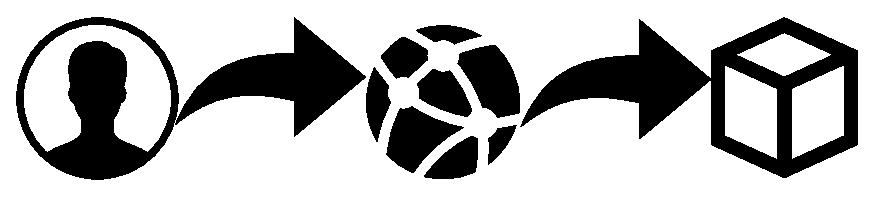
\includegraphics[width=0.5\textwidth]{figs/example.eps}
	\caption{Example of Figure.}
\end{figure}



\input{sections/04_results}
%\input{sections/05_conclusions}
\section{Planning tasks}

In this section we will shortly discuss the planning of the study. The study has been split into six parts, as can be seen in the table below. Note that this planning is merely meant as a guideline, and is not set in stone.


\noindent\resizebox{0.48\textwidth}{!}{
\begin{gantt}[xunitlength=0.5cm,fontsize=\small,titlefontsize=\small,drawledgerline=true]{13}{18} %(1)lines (2) columns
 
    \begin{ganttitle} %Month
      \titleelement{June}{4}
      \titleelement{July}{4}
      \titleelement{August}{4}
     \titleelement{September}{4}
     \titleelement{October}{2} 
    \end{ganttitle}
   
    \begin{ganttitle} % Week number
      \numtitle{23}{1}{40}{1}
    \end{ganttitle}

    \ganttbar{Proposal}{0}{2}
    
    \ganttgroup{Rel. Work}{2}{5}
    \ganttbar{task 2}{2}{2}
    \ganttbarcon[pattern=crosshatch,color=blue]{task 3}{4}{1} %(1)start point; (2) number of weeks
    \ganttbarcon{task 4}{5}{2}  
%    \ganttcon{5}{5}{6}{6} %(1)vertical bar 

   \ganttgroup{Holidays*}{7}{3}

   \ganttgroup{Analysis}{10}{6}
   \ganttbar{task 5}{10}{2}
    \ganttbarcon[color=red]{task 6}{12}{2}
    \ganttbarcon{task 7}{14}{2}
    
    \ganttmilestone{Deadline}{17}
  \end{gantt}
}


The research topics part consists solely of a literature study that focuses on ... All relevant information learned from this will be integrated in a survey that will form the first part of the thesis.

Following the research topics are each of the research questions, with time allotted at the end of each research question to integrate the results into the thesis. 

\newpage
\bibliography{bibliography}

\newpage
\newpage\newpage
\section*{IMPORTANT NOTES and TIPS:}

\begin{itemize}
	\item I DO recommend: "PhD: How to write a great research paper." \url{https://www.youtube.com/watch?v=1AYxMbYZQ1Y} (updated on 17/01/2019)
	\item Figures MUST be in svg, eps, or pdf format (I like to use Inkscape to create my figures, then I export to pdf);
	\item Graphs could be plotted using gnuplot but I prefer anything from jupyter notebook; 
	\item Avoid vague words: relatively, possible, ... 
	\item Be quantitative! give an idea of numbers.
	\item Avoid start with 'because'
	\item To reference something you can do like this: \citep{justyna2015SBRC}, \citep{kerkers2014aims}, or \citet{jjsantanna2015IM2,jjsantanna2015IM1}, \citet{santanna2013aims} \comment{Look how I did in the latex file}

\end{itemize}



\end{document}
